% TODO: images are on counted
\section{ЗАДАЧІ МАРКЕТИНГОВОЇ РОЗВІДКИ ТА МОДЕЛЮВАННЯ МАРКЕТИНГОВИХ КАНАЛІВ}
% Ми не створюємо канал як такий. Метою роботи є маркетингове прогнозування 
% шляхом моделювання маркетингового каналу.
%
% TODO: можливо, заголовок треба буде змінити
% TODO: додати новий сорець
\subsection{Основні проблемі розробки програмних систем}
\subsubsection{Основні поняття}
% TODO: програмна інженерія
% TODO: програмне забезпечення
% TODO: системна вимога
% TODO: програмний засіб
% TODO: системні вимоги
% TODO: проблемна область  
\subsubsection{Необхідність створення ПС}
\subsubsection{Процес розробки ПЗ}
% TODO: МЖЦ, методології
\subsubsection{Нотація, що використовується}
% TODO: UML, IDEF*

\subsection{Маркетингові інформаційні системи}
\subsubsection{Необхідність створення МІС}
%    Компанії зростають, роль маркетологів зростає.
Кожна зростаюча компанія коли-небудь зтикається з необхідністю розробки маркетингової стратегії та планування маркетингової діяльності відповідно до розробленої стратегії. Маркетингова стратегія --- це процес, що дозволяє компанії досягати росту продажів та сталих конкурентних переваг, концентруючи ресурси тільки на оптимальних можливостях\cite{baker}. За рішення про вибір та використання ринкових можливостей компанії відповідає маркетинговий підрозділ компанії. 
 
Для підтримки прийняття рішень, маркетологи повинні бути забезпечені постійним доступом до точної та актуальної інформації про клієнтів, продажі, конкурентів тощо. В процесі збору цієї інформації виникають проблеми, що пов’язані з ростом компанії, тобто, з масштабуванням бізнес-процесів: зростають об’єми інформації, зростає час, необхідний на обробку та аналіз, зростають витрати на зберігання. Для вирішення цих проблем використовують системи підтримки прийняття рішень, до яких відносять і маркетингові інформаційні системи. Маркетингова інформаційна система або МІС (англ. {\it marketing information system, MkIS}) --- це сукупність людей та систем, що виконують процедури збору, сортування, аналізу та оцінки інформації для підтримки прийняття маркетингових рішень \cite{kotler14}. МІС може входити до складу більш загальної системи підтримки прийняття керівних рішень, EIS (англ. {\it executive information system}).
%    Але ринок дуже великий і маркетологи не справляються. Рішення приймаються дедалі важче.
%    Для підтримки прийняття рішень, треба забезпечети маркетологів інформацією => треба організувати підприємство потрібним чином.
%    MIS -- це...  входить до MIS та чогось ще.
%    
% \subsubsection{Проблеми МІС}
%    MIS складається з трьох частин:
%    Внутрішнє -- це класи систем ERP та CRM
%    Аналіз -- це вирокистання ретроспективних даних, зібраних внутрішнім обліком. Роблять аналітики
%    Маркетингова розвідка -- це..., що має на увазі: корпоративна/конкурентна розвідка
%    Проблема: відсутня система корпоративної розвідки ситуації на ринку.
%    
% \subsubsection{Корпоративна розвідка}
%    Корпоративна розвідка здійснюється наступними методами: ...
%    Пропонується робити розвідку шляхом моделювання маркетингового каналу.
%

%\subsubsection{Огляд МІС} 
% TODO: додати цю абревіацію до відповідного розділу
% TODO: тупе визначення маркетингу, не в’яжеться взгалалі. Придумати нову структуру.
%За визначенням Американської асоціації маркетингу, {\it маркетинг} --- це діяльність, сукупність інститутів і процесів, що забезпечують створення, інформування, доставку та обмін пропозицій, що мають цінність для споживачів, клієнтів, партнерів і суспільства в цілому \cite{kotler14}. Оскільки продажі є головним джерелом прибутку, компанії будують свою структуру та процеси з оглядом на потреби маркетингу, потреби ринку. Для прийняття ефективних маркетингових рішень, компанії організовують постійний збір та аналіз інформації про споживачів, партнерів та ринок в цілому. Для автоматизації процесу збору та аналізу, використовують системи підтримки маркетингових рішень або маркетингові інформаційні системи (МІС). Маркетингові інформаційні системи (англ. {\it marketing information systems, MkIS}) --- це сукупність людей та систем, що виконують процедури по збору, сортування, аналізу та оцінки інформації для підтримки прийняття рішень.

% TODO: що це таке, навіщо воно потрібно, складові частини та їх призначення, 4Р
\begin{stdfigure}
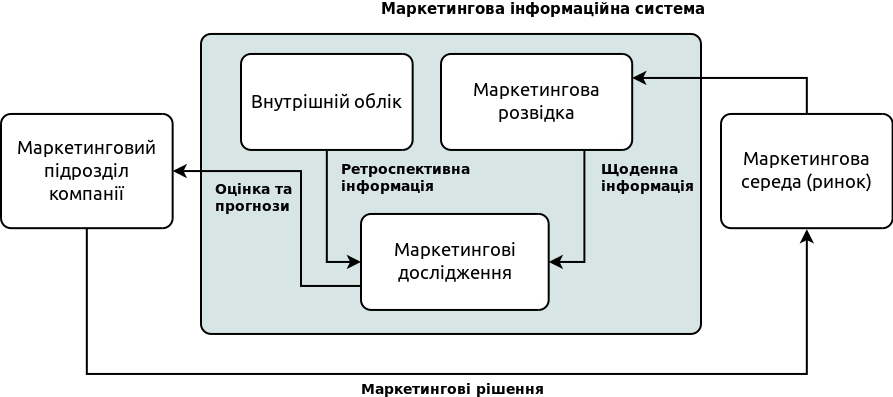
\includegraphics[width=6in]{images/mis_structure.png}
\caption{Структура МІС}
\label{fig:mis_structure}
\end{stdfigure}
 
Маркетингова інформаційна система складається з трьох частин (див. рис. \ref{fig:mis_structure}): 
\begin{itemize}
\item Внутрішній облік.
\item Маркетингові дослідження
\item Маркетингова розвідка
\end{itemize}
% Дати визначення (із посиланням на 14-те видання)
% Вставити зображення зі схемою.
% Надати опис усім трьом частинам, остання та найдетальніша: розвідка.
% TODO: що це таке, навіщо воно потрібно, складові частини та їх призначення, 4Р


\subsubsection{Маркетингова розвідка}
% TODO: Що то, нащо треба, як це робиться (моделювання, дослідження, etc), огляд наявних систем

\subsubsection{Бізнес-ігри}
% TODO: що таке бізнес-ігри, навіщо вони потрібні і як реалізються

\subsection{Постановка задачі}
\subsubsection{Моделювання маркетингового каналу}
%TODO: що таке концепція маркетингового каналу, основні момент структури та керування каналом.
% TODO: постановка задачі моделювання ()

\subsubsection{Вимоги до програмного забезпечення}